%%%%%%%%%%%%%%%%%%%%%%%%%%%%%%%%%%%%%%%%%
% Design based on a template by Roberto and following the format of
% the xmipp tutorials. In turn, they seem to be based on a template
% from http://www.latextemplates.com
%%%%%%%%%%%%%%%%%%%%%%%%%%%%%%%%%%%%%%%%%

%----------------------------------------------------------------------------------------
%	PACKAGES AND OTHER DOCUMENT CONFIGURATIONS
%----------------------------------------------------------------------------------------

\documentclass[12pt]{article} % Default font size is 12pt, it can be changed here
\usepackage[english]{babel}
\usepackage[utf8]{inputenc}
\usepackage{listings} % To include source code
\usepackage{caption}
\usepackage{geometry} % Required to change the page size to A4
%\geometry{a4paper} % Set the page size to be A4 as opposed to the default US Letter
\usepackage{framed}
\usepackage{url}
\usepackage{graphicx} % Required for including pictures
\usepackage{natbib}
\usepackage{float} % Allows putting an [H] in \begin{figure} to specify the exact location of the figure
\usepackage{hyperref}
\usepackage{menukeys}

\usepackage{fancyhdr}
\pagestyle{fancy}
\fancyhf{}
\fancyhead[RO]{{Introductory Tutorial}}
\fancyhead[LO]{Scipion}
%\fancyhead[RO]{{\leftmark}}
\fancyfoot[RO]{\thepage}

\linespread{1.2} % Line spacing

%\setlength\parindent{0pt} % Uncomment to remove all indentation from paragraphs

\newcommand{\scipion}{\textsc{Scipion} }
\newenvironment{command}{\tt\begin{quote}}{\end{quote}}
\newcommand{\comm}[1]{\texttt{#1}}

\begin{document}


%----------------------------------------------------------------------------------------
%	TITLE PAGE
%----------------------------------------------------------------------------------------

\begin{titlepage}

% New command for horizontal lines. Change thickness here.
\newcommand{\HRule}{\rule{\linewidth}{0.5mm}}

\center % Center everything on the page


\includegraphics{../tutorial_common/images/scipion_logo.png}

{\large Scipion Tutorial Series}\\[1.0cm]

\textsc{\LARGE National Center for Biotechnology}\\[0.5cm]
\textsc{\Large Biocomputing Unit}\\[0.5cm]

\HRule\\[0.4cm]
{ \huge \bfseries Introductory Tutorial}\\[0.4cm] % Title of your document
\HRule \\[1.5cm]

%{\large \today}\\[3cm] % Date, change the \today to a set date if you want to be precise

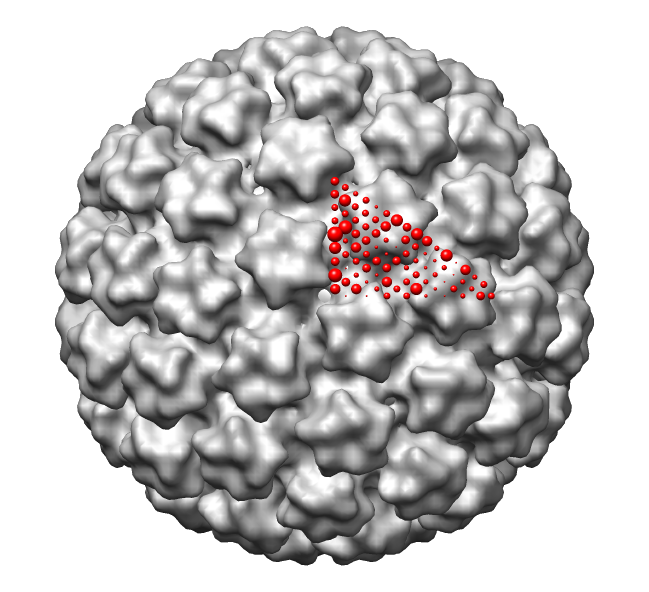
\includegraphics[width=0.5\textwidth]{{images/13.VolumeChimeraAndProjections}.png}

\vfill % Fill the rest of the page with whitespace
%\begin{minipage}{0.4\textwidth}
\begin{flushright}
 \large
%\emph{Author:}\\
  \textsc{Scipion Team} % Your name
\end{flushright}
%\end{minipage}

\end{titlepage}


%----------------------------------------------------------------------------------------
%	OBJETIVOS
%----------------------------------------------------------------------------------------


\subsection*{Intended audience}

This tutorial provides a general introduction to Scipion, an image
processing framework to obtain 3D models of macromolecular complexes
using Electron Microscopy (EM). It is designed to introduce 3D image
processing in EM to people without any prior knowledge of Scipion,
some limited knowledge about 3D-EM image processing, and basic
computer skills.

\subsection*{We'd like to hear from you}

We have tested and verified the different steps described in this demo
to the best of our knowledge, but since our programs are in continuous
development you may find inaccuracies and errors in this text. Please
let us know about any errors, as well as your suggestions for
future editions, by writing to
\href{mailto:scipion@cnb.csic.es}{scipion@cnb.csic.es}.

\newpage


%----------------------------------------------------------------------------------------
%	TABLE OF CONTENTS
%----------------------------------------------------------------------------------------

\tableofcontents % Include a table of contents

\newpage % Begins on a new page instead of on the same page as the table of contents


\section{Software Installation}

The first step is to download %before starting to work on your projects is to download
and install \scipion and related software packages. We describe
briefly the process in the next sections. For the full documentation please refer to
\url{http://scipionwiki.cnb.csic.es/bin/view/TWiki/NewInstallation}.

\subsection{Xmipp}

Xmipp is one of the main EM software packages supported in \scipion. To download
%One of the main components of \scipion is the Xmipp package. To get
the latest version use:

\begin{command}
git clone http://git.code.sf.net/p/newxmipp/code xmipp
\end{command}

\noindent
then change to the \directory{xmipp} directory and run the installation with

\begin{command}
./install.sh
\end{command}

%\subsection{Scipion and Extra Packages}
\subsection{Scipion}

To get the latest version of \scipion run

\begin{command}
git clone http://git.code.sf.net/p/pyworkflow/code scipion
\end{command}

\noindent
and then change into the \directory{scipion} directory. Finally run:

\begin{command}
./scipion install --with-all-packages --with-xmipp=\$XMIPP\_HOME
\end{command}

\noindent
where \verb+$XMIPP_HOME+ points to the directory with your local
installation of Xmipp.


\section{Reconstruction of a Viral Capsid}

In this demo, we use the \emph{single particle analysis} approach to obtain
a 3D reconstruction of a \emph{Bovine Papillomavirus}. The EM images have been kindly
provided by \href{http://grigoriefflab.janelia.org/}{Dr.~Grigorieff’s Lab}. Micrographs were
collected at 300 $kV$ and a calibrated magnification of 56,588,
giving a pixel
size of 1.237 \AA  \citep{Wolf2010}. 

\subsection{Getting Started}

To download the data required for this tutorial use the following command:

\begin{command}
scipion testdata --download xmipp\_tutorial
\end{command}

\noindent
It will be downloaded to \$\directory{SCIPION\_HOME/data/tests}. 

To start image processing in \scipion we need to run \comm{scipion} from the command line.
For this tutorial we register a new project by clicking the \keys{Create Project}
button and specifying project name. Then we navigate to project window (Figure \ref{fig:Project}).  
Left panel displays possible workflows, such as Single Particle Analysis (SPA) or Random Conical Tilt (RCT), 
and its different reconstruction tasks listing protocols available.
Top right panel displays the sequence of protocols executed by the user and its state: running, finished, aborted. Users can visualize it using list or tree views.
Finally bottom right panel displays information for the selected run, such as inputs and outputs, execution logs or documentation - also provides "Analyze Results" button to visualize outputs.

\begin{figure}[H]
\centering
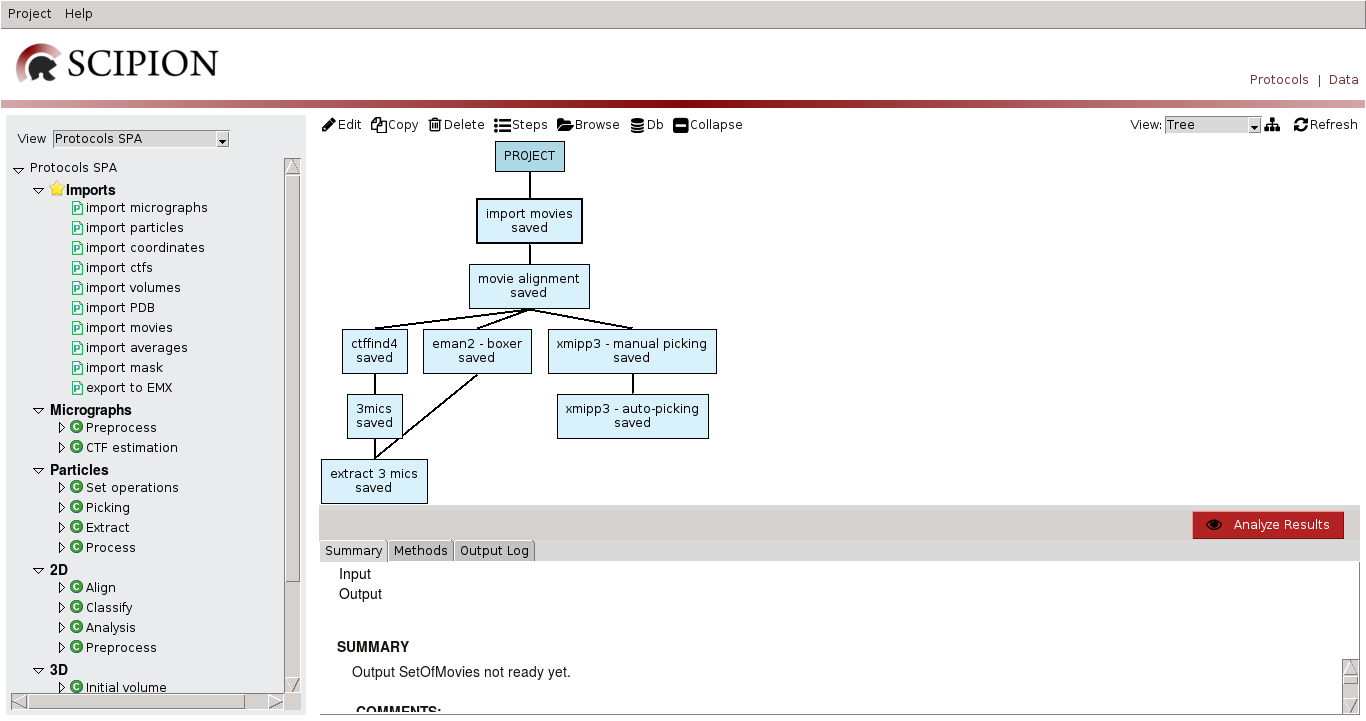
\includegraphics[width=0.7\textwidth]
{{images/00.Project}.png}
\caption{Project window}
\label{fig:Project}
\end{figure}


\subsection{Preprocessing}

\subsubsection{Importing Micrographs}

The first step is to import the micrographs to your scipion
project. To do this, double-click the \keys{Import Micrographs}
button. In \textit{Pattern} indicate where your micrograph files are
stored (for example by clicking on the browse button, the one
that looks like a folder). The complete pattern
is:\\
\verb+$SCIPION_HOME/data/tests/xmipp_tutorial/micrographs/*.mrc+

Modify the parameters of the Import Micrographs protocol according to
the ones shown in figure (\ref{fig:ImportMics}).  Then click on the
\keys{Save} and \keys{Execute} buttons. After executing the
protocol, the project window will present the new information as shown in
figure (\ref{fig:ProjectGUI}).

\begin{figure}
\centering
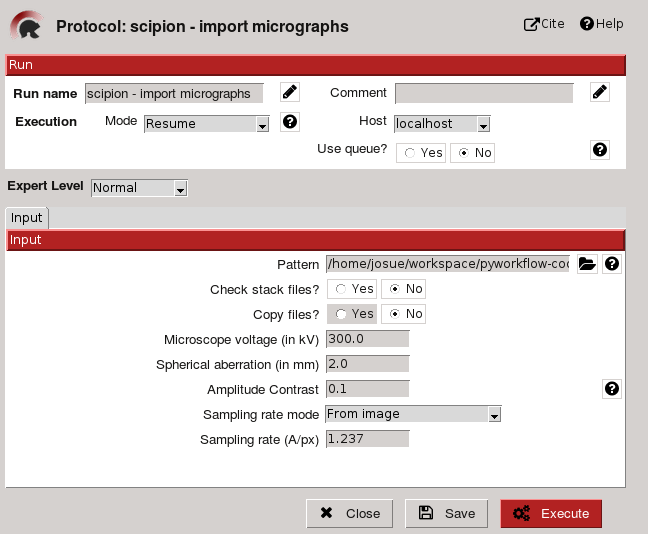
\includegraphics[width=0.7\textwidth]
{{images/01.Import_Mics}.png}
\caption{Import Micrographs protocol dialog.}
\label{fig:ImportMics}
\end{figure}

\begin{figure}
\centering
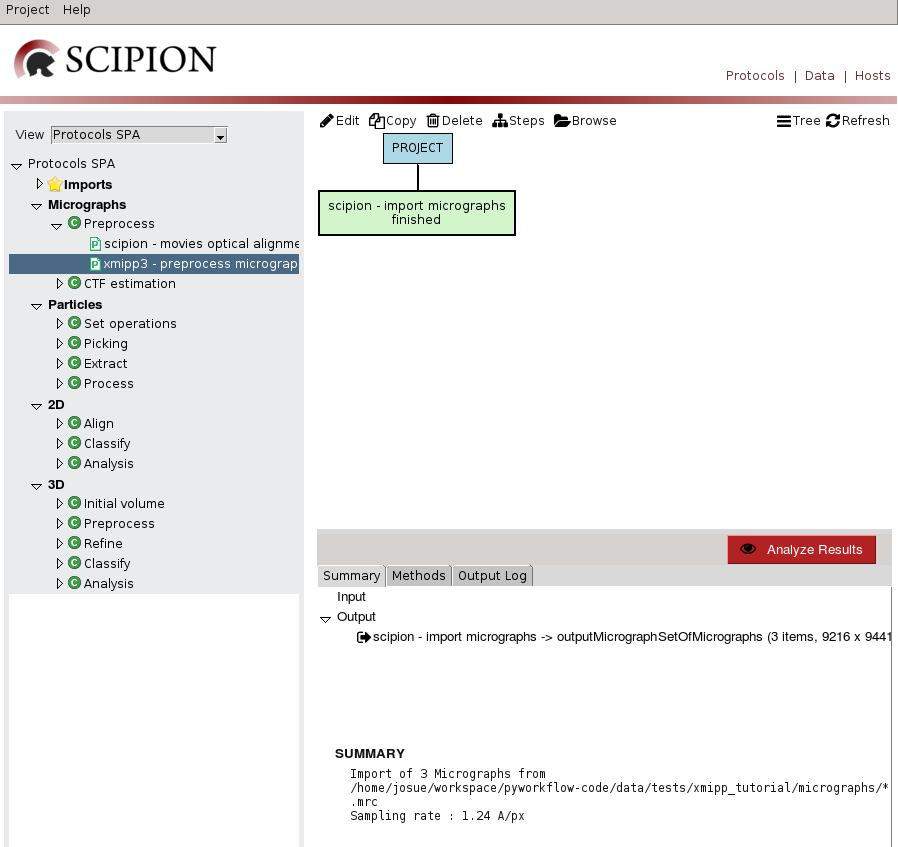
\includegraphics[width=0.9\textwidth]{{images/02.Project_GUI}.png}
\caption{Scipion project GUI after processing Import Micrograph protocol.}
\label{fig:ProjectGUI}
\end{figure}

If we press the \keys{Analyze Results} button a new dialog will
appear that shows the different imported micrographs (not shown).

\subsubsection{Downsampling Micrographs}

After importing the micrographs to your \scipion project, you can
perform the next step: \textbf{Preprocess Micrographs}. This protocol
combines multiple Xmipp programs in order to perform several operations
over the micrographs. Double-click on the protocol name and fill the
dialog with the options shown in figure (\ref{fig:Preprocess}). To
fill the \textit{Input micrographs} field, simply click on the
magnifying glass button and select the output from the previous step.

\begin{figure}
\centering
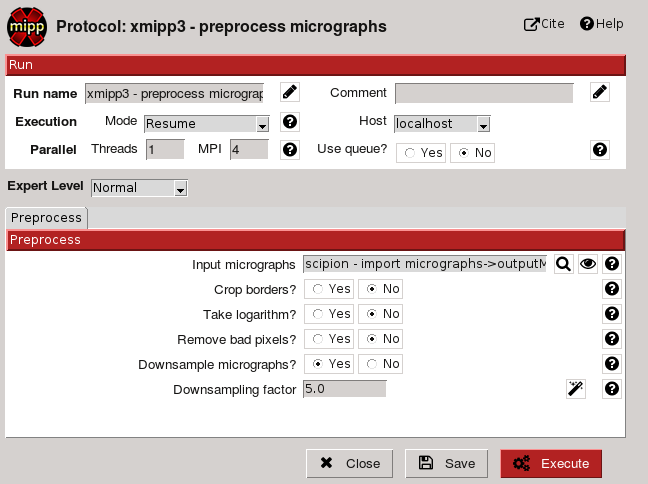
\includegraphics[width=0.75\textwidth]{{images/03.Downsampling_Mics}.png}
\caption{Preprocess Micrographs dialog.}
\label{fig:Preprocess}
\end{figure}

\subsubsection{CTF Estimation}

The next step is to estimate the CTFs (Contrast Transfer Functions) of
the micrographs. There are currently two protocols in \scipion to
estimate the CTF: \textit{CTFFind} \citep{Mindell2003} and
\textit{Xmipp CTF estimation}. You don't need to do any extra work to use
both programs, like changing the extension of the micrographs, because
in \scipion the inputs and outputs that belong to the same type of
protocol are standarized.

These protocols estimate the PSD (Power Spectral Density) of the
micrographs to then estimate the parameters of the CTF (defocus U,
defocus V, defocus angle, etc).  They cut the micrographs into plenty
of images with the desired size. After that, they compute the Fourier
Transform of each image and make an average.

\begin{description}

\item[CTFFind] \hfill \\
To estimate the CTF with CTFFind, you will need some parameters
describing the frequency region to be analyzed. The parameters shown
in figure (\ref{fig:CTFFind}) are the proper ones for this example.
The limiting frequencies must be such that all zeros of the PSD are
contained within those frequencies. There is a wizard, shown in figure
(\ref{fig:CTFwizard}), that helps in choosing those frequencies. To
see the full available options, choose the \verb+Rxpert Level+ in the
dropdown menu.  Please note that the range of defocus search is
usually larger than the one used in this example, and it must be
chosen according to your data set.

\item[Xmipp CTF estimation] \hfill \\
If you prefer, you can estimate the CTF with the
Xmipp CTF estimation. The parameters used in this protocol are the same as
the ones in the CTFFind protocol, explained above.

\end{description}

\begin{figure}
\minipage{0.47\textwidth}
  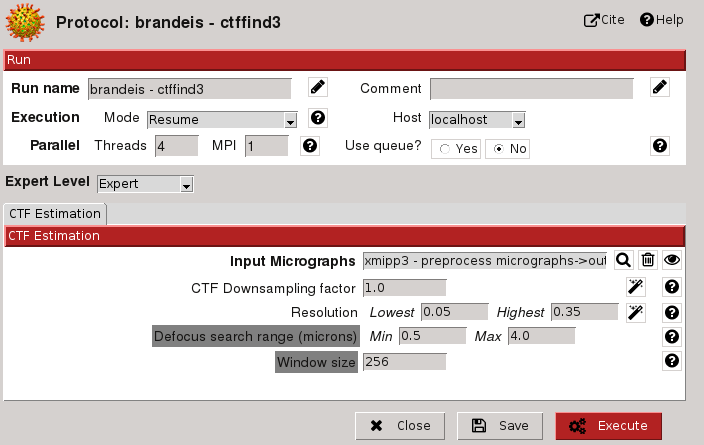
\includegraphics[width=\linewidth]{{images/04.CTFFind}.png}
  \caption{CTFFind protocol dialog.}
  \label{fig:CTFFind}
\endminipage\hfill
\minipage{0.51\textwidth}
  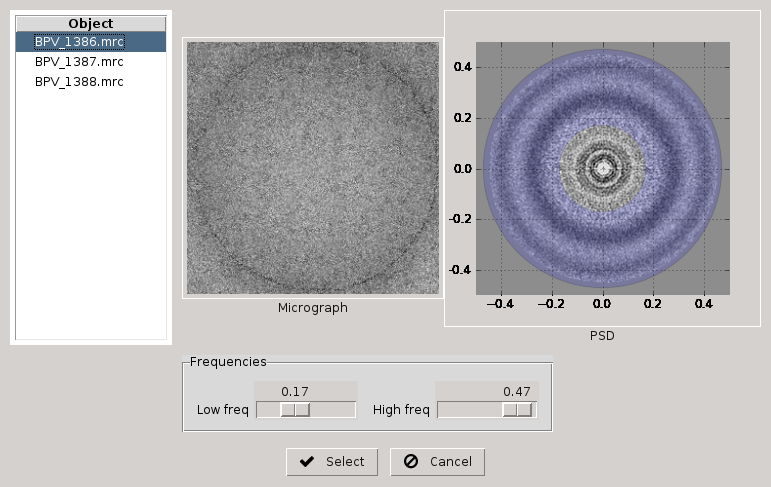
\includegraphics[width=\linewidth]{{images/16.CTFWizard}.png}
  \caption{Wizard to choose the frequencies.}
  \label{fig:CTFwizard}
\endminipage\hfill
\end{figure}

The CTFs of good micrographs typically have multiple concentric rings, shown
in figure (\ref{fig:CTFs}) left, extending from the image center towards its edges.
Bad micrographs may lack rings or have very few rings that hardly extend from
the image center. A reason to discard micrographs may be the presence of
strongly asymmetric rings (astigmatism, figure (\ref{fig:CTFs}) center) or rings
that fade in a particular direction (drift, figure (\ref{fig:CTFs}) right).

\begin{figure}
\centering
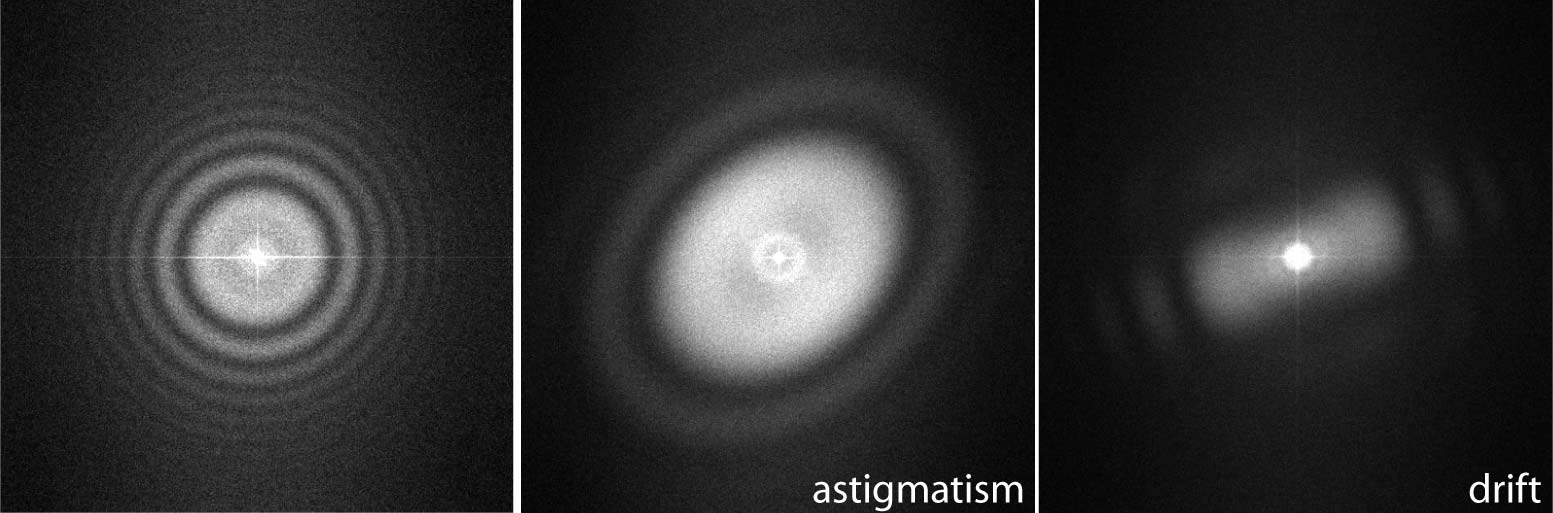
\includegraphics[width=0.75\textwidth]{images/images-016.jpg}
\caption{CTFs of good, astigmatic and drift micrographs respectively.}
\label{fig:CTFs}
\end{figure}

When the protocol (either CTFFind or Xmipp CTF estimation) is finished
you may click on the \keys{Analyze Results} button (figure
(\ref{fig:CTFResult})). To discard micrographs with bad CTFs you may
click with the mouse right button and press \textbf{Disable}. Once you
finish the selection, press on the \keys{Micrographs} button to
create your subset of micrographs with only the enabled ones.

Sometimes the CTF estimation algorithm may fail to find the rings even
if they can be seen by eye. If this is the case, you may help the
algorithm to find the rings by clicking on the image with the mouse
right-button and choosing \textbf{Recalculate CTF} on the menu that
appears. A graphical interface will help you to correctly identify the
CTF. You must provide the first CTF zero and the limits, and then
press \verb+OK+. When you finish, press the \keys{Recalculate CTFs}
button.

\begin{figure}
\centering
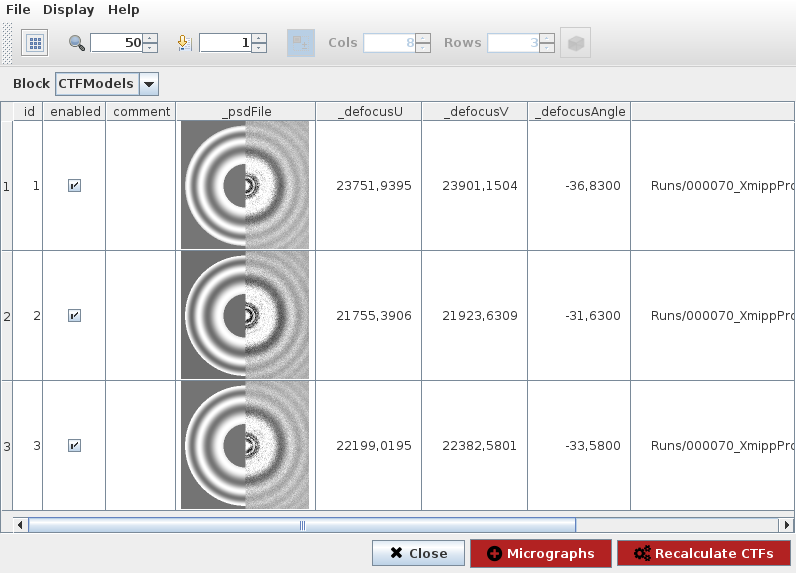
\includegraphics[width=0.75\textwidth]{{images/17.CTFREsults}.png}
\caption{Output visualization of the CTFFind protocol that shows the
CTFs of all the micrographs, and different related parameters.}
\label{fig:CTFResult}
\end{figure}

\subsubsection{Particle Picking}

Now you are ready to pick the particles. You can pick the particles in
the micrographs with either \textit{Xmipp manual picking},
\textit{Eman boxer} or the \textit{bshow} protocol. These protocols
are in interactive mode, i.e.~you can create different sets of
coordinates within the same protocol.

\begin{description}

\item[EMAN boxer] \hfill \\
Double-clicking on eman2 boxer will launch the window shown in figure
(\ref{fig:EmanProtocol}). Set the paramaters as they appear in the figure.

\begin{figure}
\centering
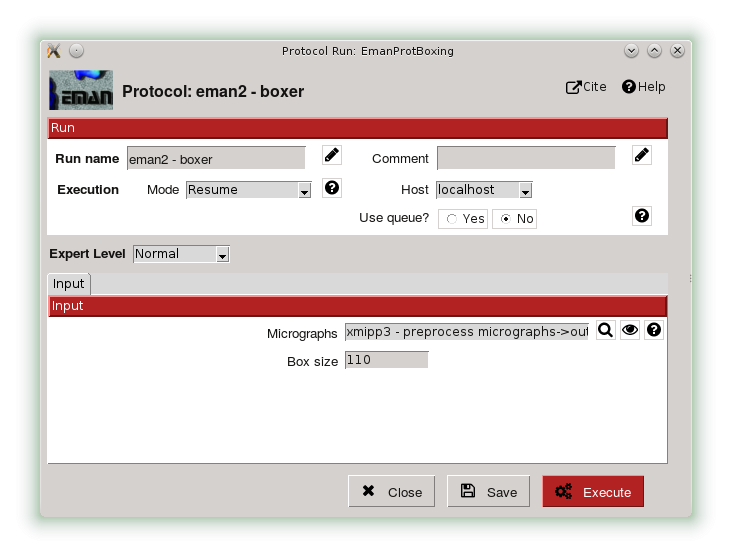
\includegraphics[width=0.75\textwidth]{{images/18.EmanPP}.png}
\caption{EMAN boxer protocol dialog.}
\label{fig:EmanProtocol}
\end{figure}

Once you press the \keys{Execute} button, several windows will open
(figure (\ref{fig:EmanPP})). This protocol has several modes of
selection, please refer to its
\href{http://blake.bcm.edu/emanwiki/EMAN2}{webpage} for futher
information. When you are done picking particles press \keys{Done}
and you will be asked if you want to create the output.  If you choose
\keys{No}, you can continue picking and the selected particles will
be added to the same Set, until you repeat the operation and say
\keys{Yes}.

\begin{figure}
\centering
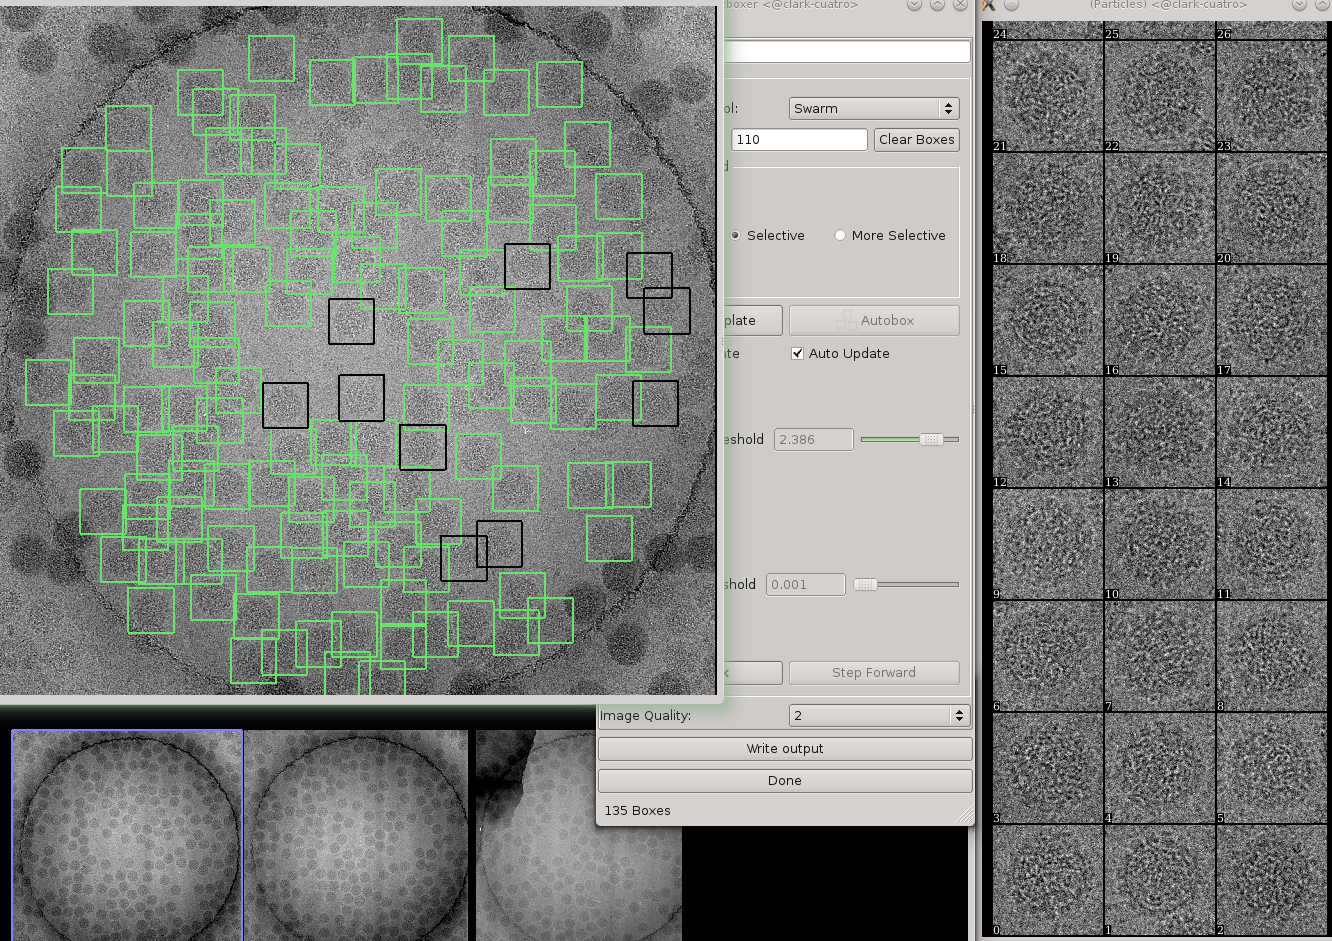
\includegraphics[width=0.75\textwidth]{{images/05.EmanPicking}.png}
\caption{EMAN boxer, an interface for particle picking.}
\label{fig:EmanPP}
\end{figure}

\item[Xmipp particle picking] \hfill \\
You could instead double-click on the \textit{Xmipp supervised
  picking} protocol. It will launch a dialog as in figure
(\ref{fig:xmipp_manual_picking}). After selecting the set of
micrographs to use and clicking \keys{Execute}, it will launch the
window shown in figure (\ref{fig:XmippPickingParticles}).

\begin{figure}
\centering
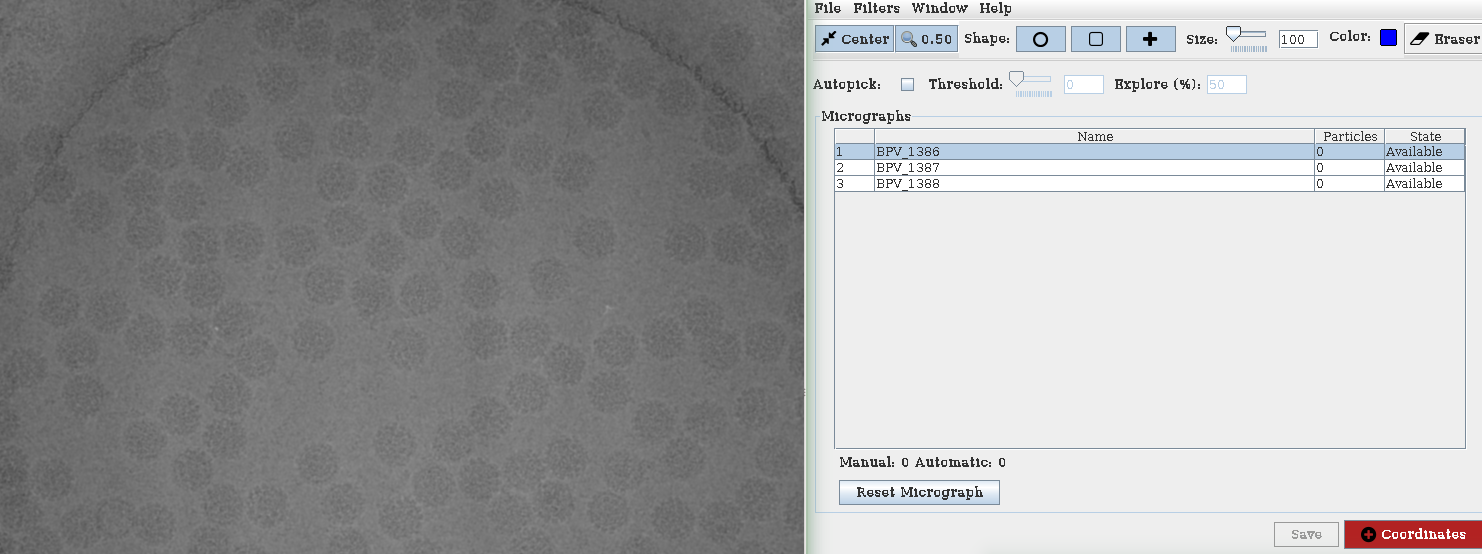
\includegraphics[width=0.75\textwidth]{{images/12-xmipp_manual_picking_protocol}.png}
\caption{Xmipp supervised picking dialog.}
\label{fig:xmipp_manual_picking}
\end{figure}

\begin{figure}
\centering
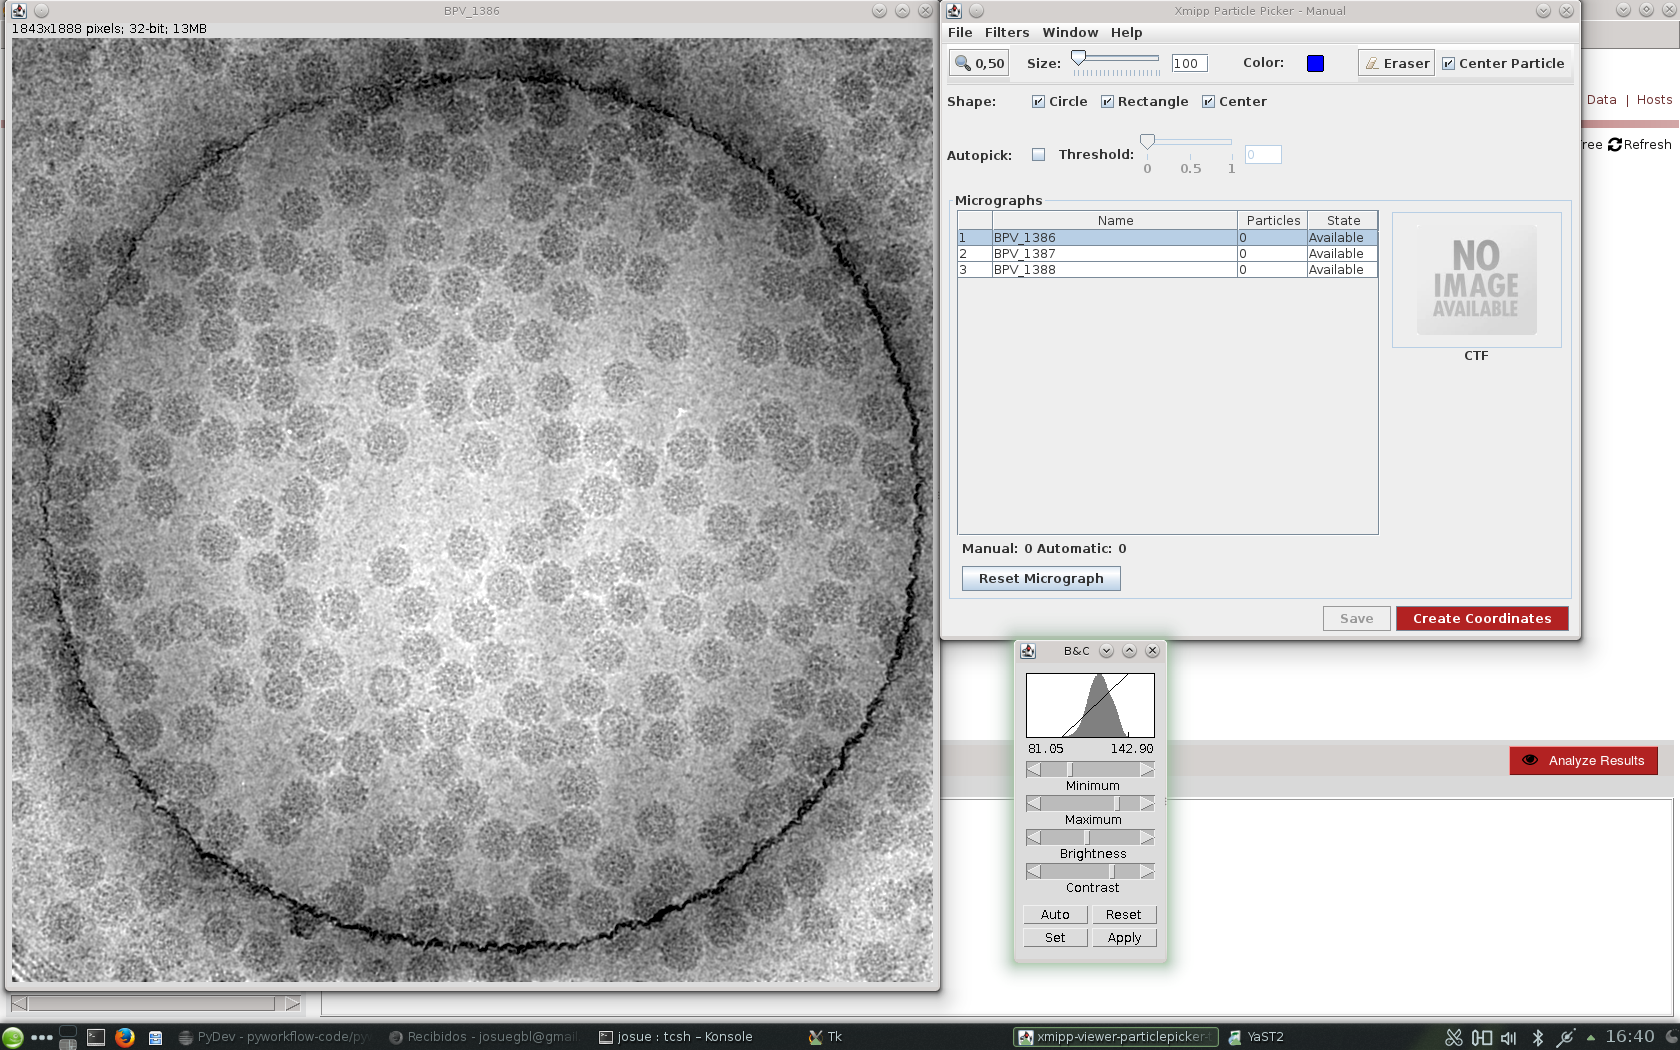
\includegraphics[width=0.75\textwidth]{{images/15.PartPickingXmipp}.png}
\caption{Xmipp supervised picking, a different interface for particle picking.}
\label{fig:XmippPickingParticles}
\end{figure}

In order to select particles:

\begin{itemize}
\item Use \keys{\shift + mouse wheel} in the overview window to zoom
  in and out.
\item Mark particles with the \keys{mouse left} button. You may move
  its position by clicking the left mouse button on the selected
  particle and dragging it to the new position.
\item Use \keys{\shift + left mouse} over a selected particle in order
  to remove it.
\item You can apply filters to the micrographs, so that you may see
  the particles better. Filters are added into a queue, so whenever
  you change the visualized area, they are applied again. Select the
  menu \menu{Filters} in the overview window and add as many filters
  as you like.
\item You can clean the filter queue, if you want to return to the
  original image.
\item You can create the set of coordinates or just save the picked
  particles to continue picking later.
\end{itemize}

\end{description}

\subsection{Extract Particles}

Click on \menu{Particles > Extract > xmipp3 - extract particles}.
This will launch the dialog of our next protocol that will allow you
to extract, normalize and correct the CTF phase of your picked
particles, among other things. Modify the default parameters according
to the ones shown in figure (\ref{fig:XmippPP}) and
(\ref{fig:ExtractParams}). They will contain:

\begin{figure}
  \centering
  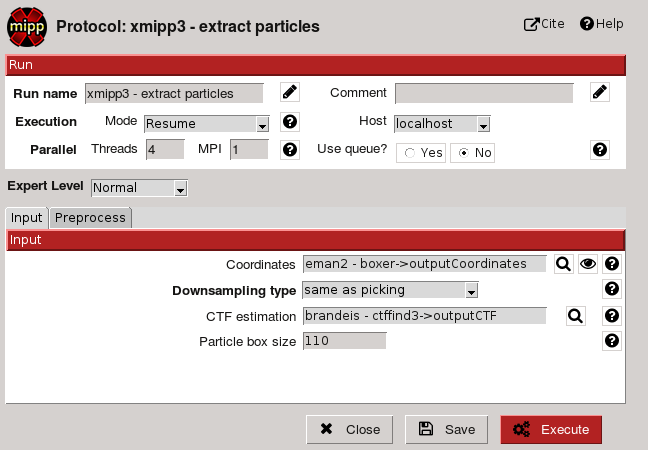
\includegraphics[width=0.75\textwidth]{{images/06.Extract_Particles}.png}
  \caption{Extract particles protocol dialog (tab \texttt{Input})}
  \label{fig:XmippPP}
\end{figure}

\begin{figure}
  \centering
  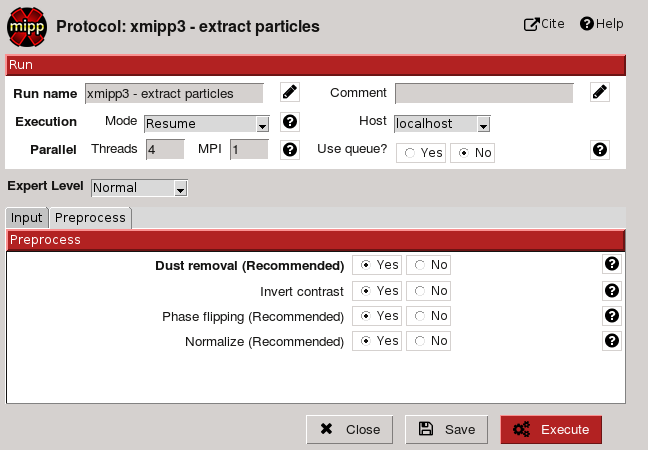
\includegraphics[width=0.75\textwidth]{{images/06.Extract_ParticlesB}.png}
  \caption{Extract particles protocol dialog (tab \texttt{Preprocess})}
  \label{fig:ExtractParams}
\end{figure}

\begin{itemize}
\item The \textit{coordinates} of the particles in the micrographs,
  which are taken from the results of the previous step. Also in the
  same tab, the \textit{particle box size} in pixels (in this case 110
  px).
\item The \textit{invert contrast} flag. If activated, bright
  regions become dark regions and the other way around. This flag
  should be set so that the extracted particles are white over a dark
  background.
\item The \textit{phase flipping} flag. If activated (recommended),
  the protocol corrects the CTF phase of your particles.
\item The \textit{normalize} flag. If activated (recommended), the
  particles are normalized to have zero mean and a standard deviation
  of one for the background pixels.
\end{itemize}


% TODO: see the definition of zscore and explain this a bit more.

The protocol also sorts the particles based on general statistics
assigning to each particle a z-score value. Particles with low z-score
are reliable and the ones with large z-score are outliers. Press the
\keys{Analyze Results} button in the main window to check the
extracted and normalized images.

\subsubsection{Particles Selection}

By default, the visualization of the particles are sorted by
z-score. If you want to remove some particles because they are
outliers and are not good particle images, press the mouse right
button on them and select \textbf{Disable}. When you are done press
the \keys{Particles} button to create a new SetOfParticles (figure
(\ref{fig:SubsetSelection})).

\begin{figure}
  \centering
  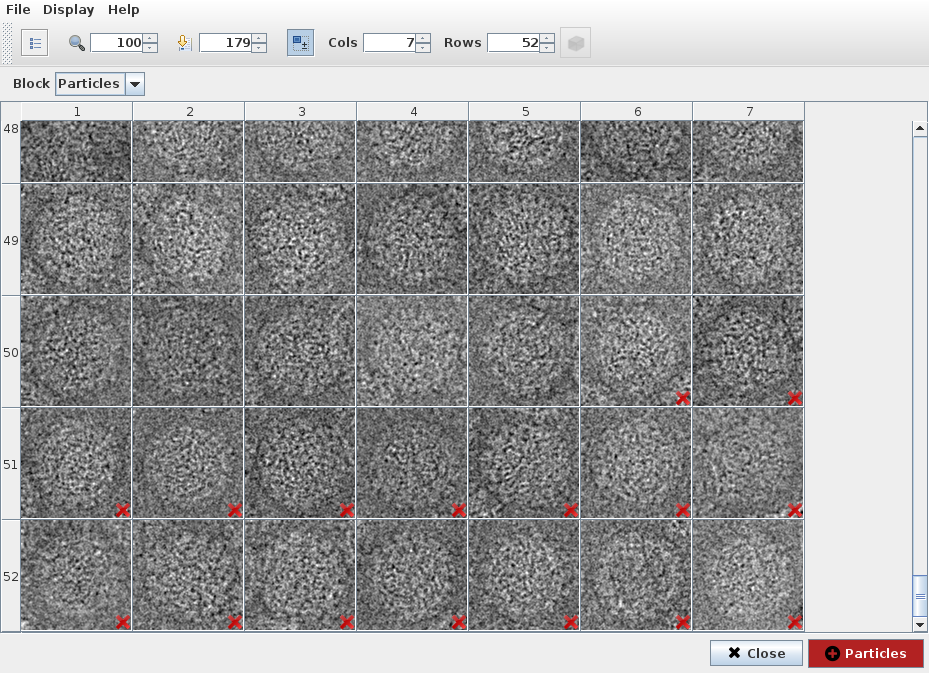
\includegraphics[width=0.75\textwidth]{{images/08.ImgsSelection}.png}
  \caption{Analyze Results window of the Extract Particles protocol.}
  \label{fig:SubsetSelection}
\end{figure}

\subsection{3D Reconstruction: Projection Matching}

Having the right angles of each projection is crucial for making a 3D
reconstruction.  However, in 3DEM you don’t know a priori the angles
and you have to estimate them as part of the problem. The most popular
way of estimating them is by comparing somehow the projections of a
volume that is similar to the volume to be reconstructed (initial
model) with the images obtained from the microscope.

A possible approach is to generate equidistant projections from the
initial model. The experimental data set is then compared (for
example, by cross correlation) to each reference projection.  A
“similarity” coefficient (for example, crosscorrelation coefficient)
is generated between each experimental particle and reference
projection. Each individual experimental particle is matched to the
reference projection that gave the highest “similarity”
coefficient. Therefore, it is assumed that this experimental particle
was projected with the same Euler angles as the reference projection.

As an initial map is necessary, you need to import a volume. Press on
\textbf{Import Volume} and set in \textit{Pattern} parameter the
following path:

% TODO: explain where. Which dialog? which menu?
% Maybe it's \menu{3D > Preprocess > xmipp3 - preprocess volumes}
% but I don't know.

% TODO: acutally, from this point below (and the last paragraph), it
% is not clear where to click on things, or how the flow is going. I
% think it should be revisited.


\begin{verbatim}
$SCIPION_HOME/data/tests/xmipp_tutorial/micrographs/BPV_scale_filtered_windowed_110.vol
\end{verbatim}

Please, set 6.185 on the \textit{sampling rate} parameter.

In order to lauch the projection matching protocol click on
\textbf{refine > projection matching} and set the parameters as the
ones shown in figures (\ref{fig:ProjMatchA}), (\ref{fig:ProjMatchB}),
(\ref{fig:ProjMatchC}) and (\ref{fig:ProjMatchD}). Choose the
SetOfParticles that has been selected previously in subset selection
protocol.

 \begin{figure}
  \centering
  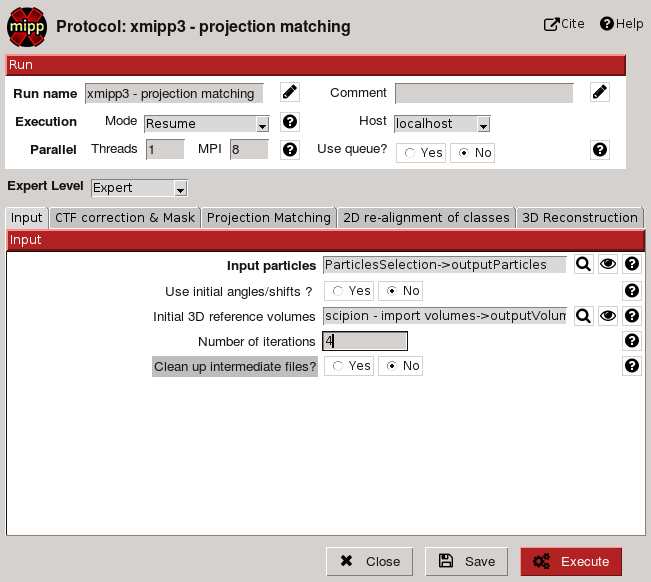
\includegraphics[width=0.75\textwidth]{{images/09.ProjMatchA}.png}
  \caption{Projection matching parameters I}
  \label{fig:ProjMatchA}
 \end{figure}

 \begin{figure}
  \centering
  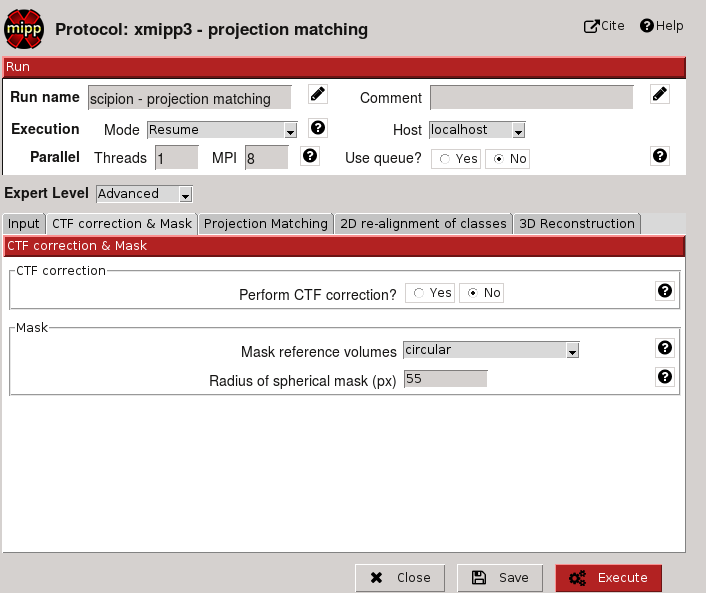
\includegraphics[width=0.75\textwidth]{{images/09.ProjMatchB}.png}
  \caption{Projection matching parameters II}
  \label{fig:ProjMatchB}
 \end{figure}

  \begin{figure}
  \centering
  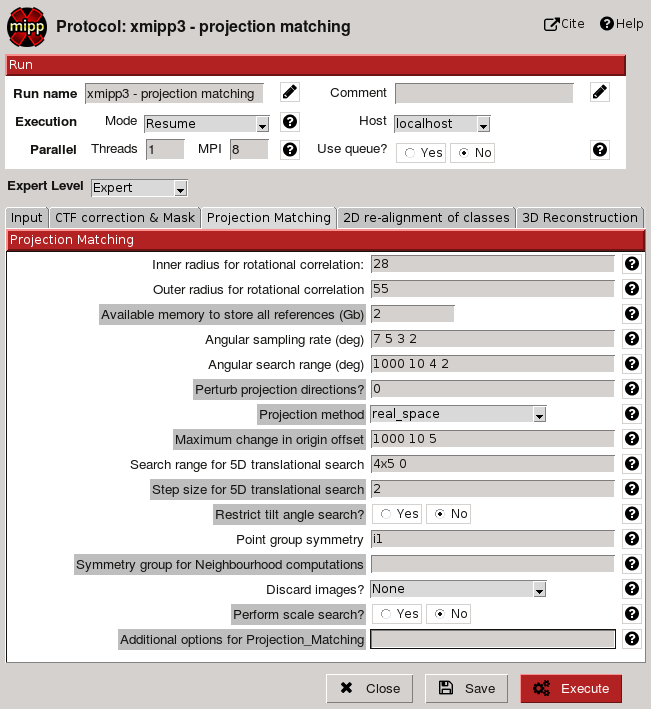
\includegraphics[width=0.75\textwidth]{{images/09.ProjMatchC}.png}
  \caption{Projection matching parameters III}
  \label{fig:ProjMatchC}
 \end{figure}

  \begin{figure}
  \centering
  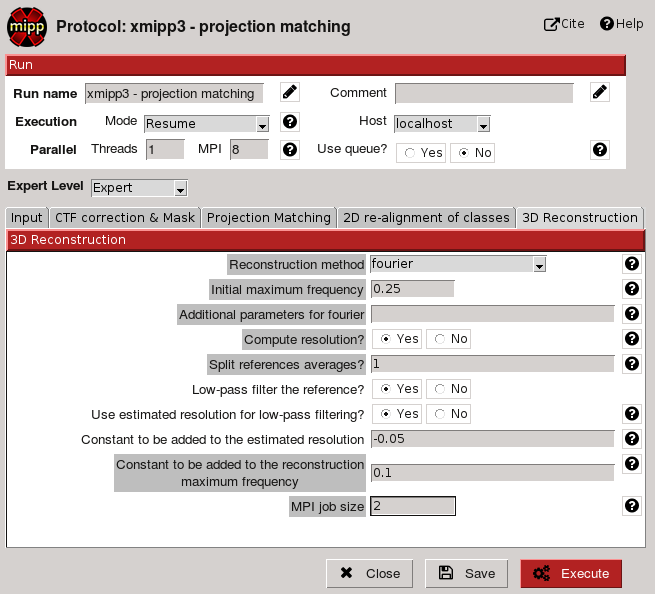
\includegraphics[width=0.75\textwidth]{{images/09.ProjMatchD}.png}
  \caption{Projection matching parameters IV}
  \label{fig:ProjMatchD}
 \end{figure}

Finally, in order to visualize the obtained results click on
\textbf{Analyze Results} button. You will see a GUI as the one shown in
figure (\ref{fig:ProjMatchViewer}).

 \begin{figure}
  \centering
  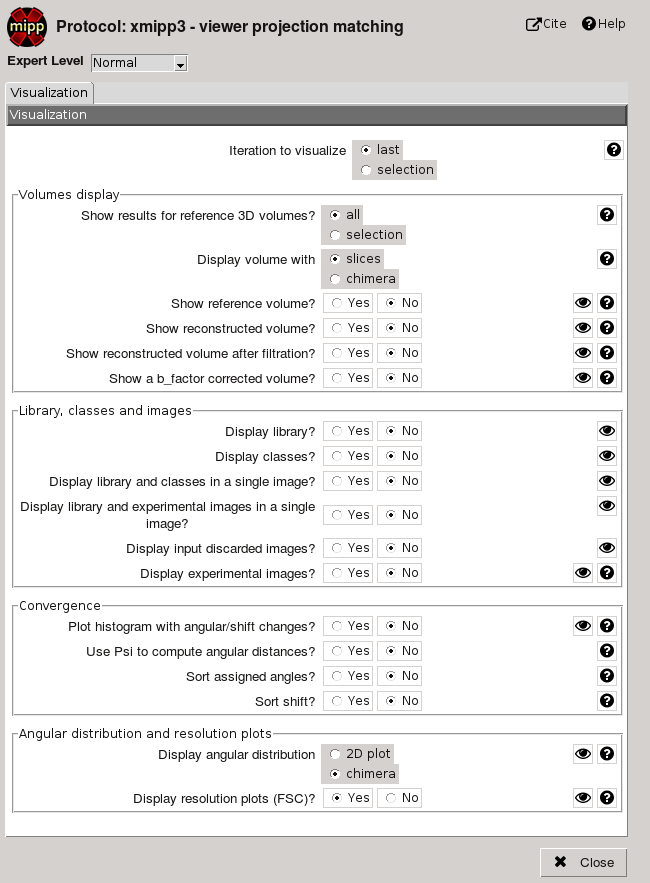
\includegraphics[width=0.75\textwidth]{{images/11.ProjMatchViewer}.png}
  \caption{Projection matching viewer}
  \label{fig:ProjMatchViewer}
 \end{figure}

To see the volumes you can press \textbf{eye} button in the field
\textit{Display reconstructed volume?} and you will see the reconstructed
volume as shown in figure (\ref{fig:volShowj}) or in chimera if you select Chimera
checkbox (figure (\ref{fig:volChimera})).

 \begin{figure}
  \centering
  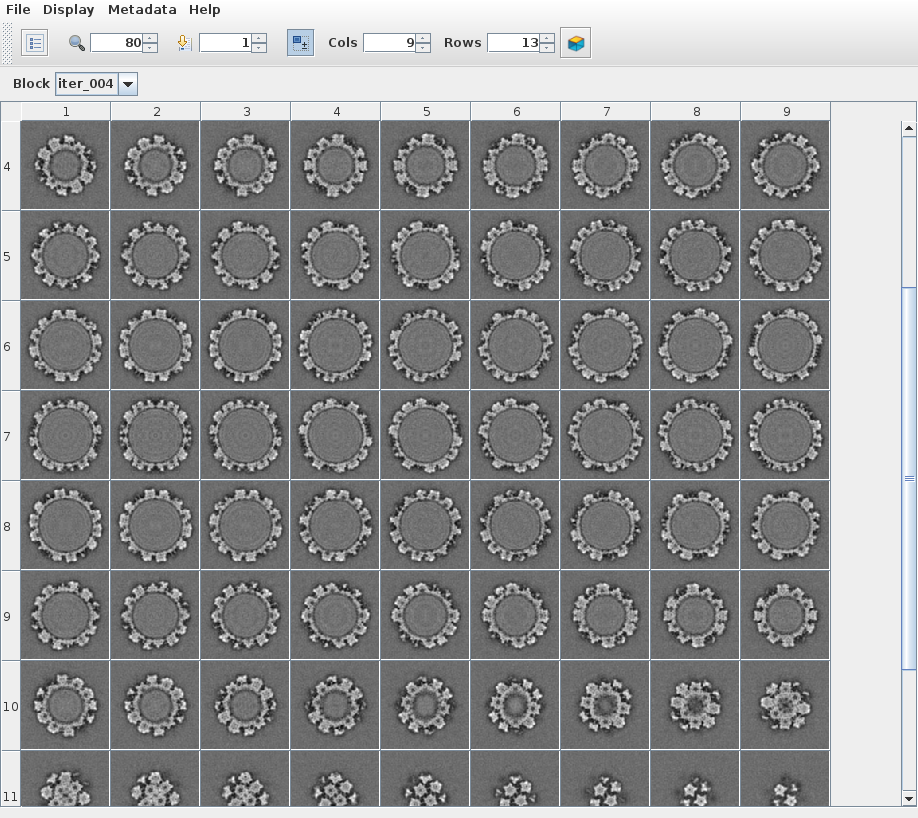
\includegraphics[width=0.75\textwidth]{{images/12.VolumeGalleries}.png}
  \caption{reconstructed volume}
  \label{fig:volShowj}
 \end{figure}

 \begin{figure}
  \centering
  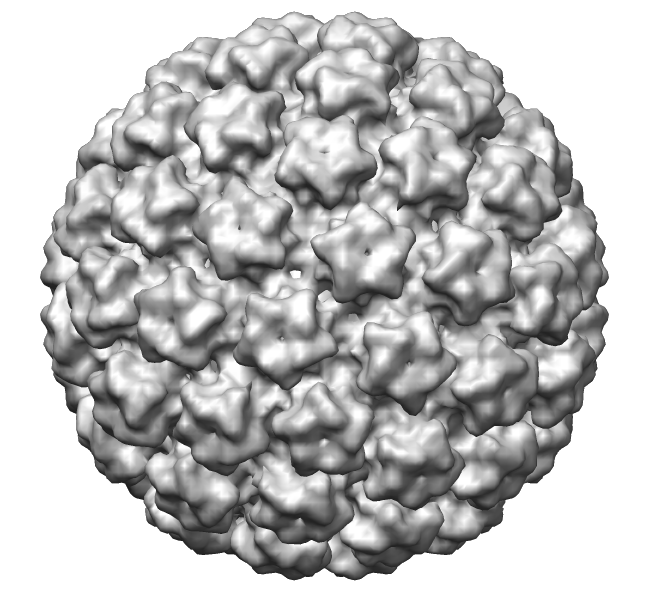
\includegraphics[width=0.75\textwidth]{{images/12.VolumeChimera}.png}
  \caption{reconstructed volume with chimera}
  \label{fig:volChimera}
 \end{figure}

\subsection{Frealign Refinement}

 If you want to refine the output volume of projection matching, you can
 use Frealign refinement protocol. First, you need the "same" SetOfParticles
 that has been processes with Projection matching, but with the features needed
 to Frealign.

 \begin{description}
  \item [Subset selection:]  To do this, the firs step is extract the particles
  again, but Preprocess tab changed as shown in figure (\ref{fig:ExtractForFrealign}).

  \begin{figure}
   \centering
   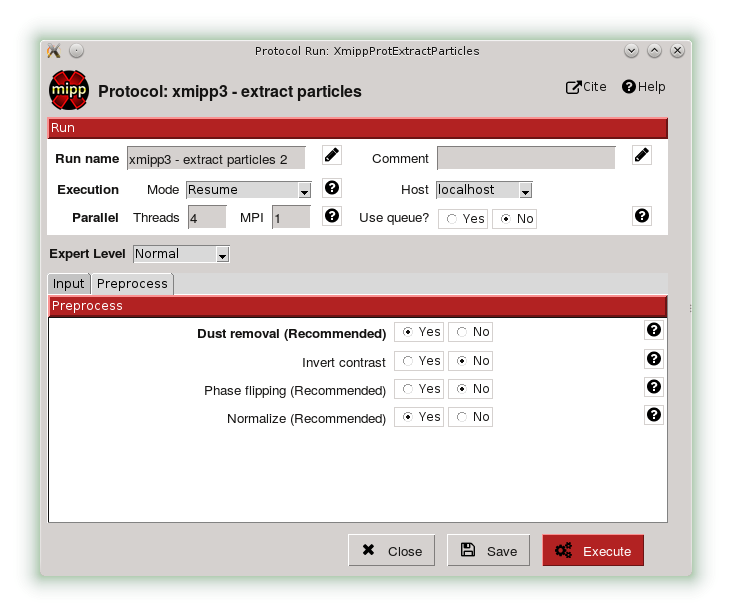
\includegraphics[width=0.75\textwidth]{{images/06.Extract_ParticlesC}.png}
   \caption{GUI of Extract Particles protocol II}
   \label{fig:ExtractForFrealign}
 \end{figure}

 Once the particles are extracted, press on \textbf{Set operations $\rightarrow$ intersect sets}
 button. In first place, you set the last Extracted particles, and in second place
 the particles selected that has been used to refine a 3D reconstruction.
  \end{description}


The new SetOfParticles is the input of Frealign refinement
protocol. Please, set the parameters as shown in figures
(\ref{fig:FrealignA}), (\ref{fig:FrealignB}), (\ref{fig:FrealignC})
and (\ref{fig:FrealignD}).

 \begin{figure}
  \centering
  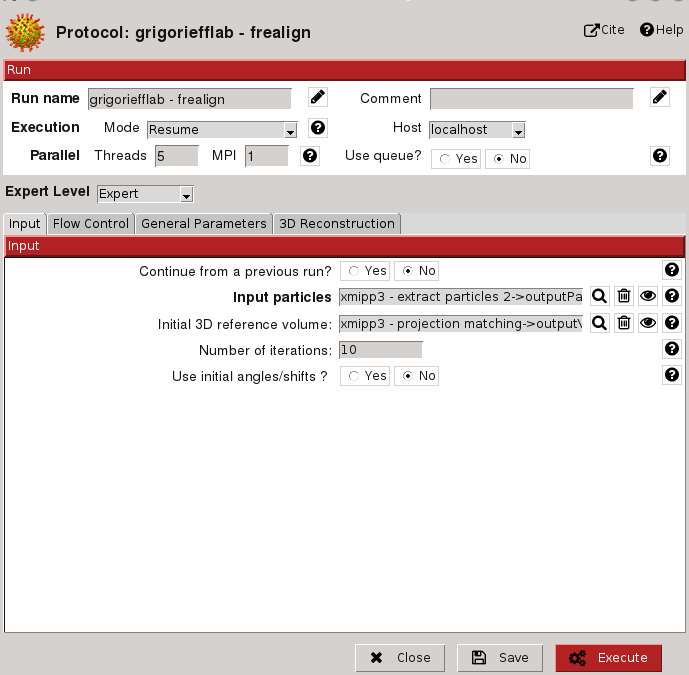
\includegraphics[width=0.75\textwidth]{{images/19.FrealignA}.png}
  \caption{Frealign parameters I}
  \label{fig:FrealignA}
 \end{figure}

 \begin{figure}
  \centering
  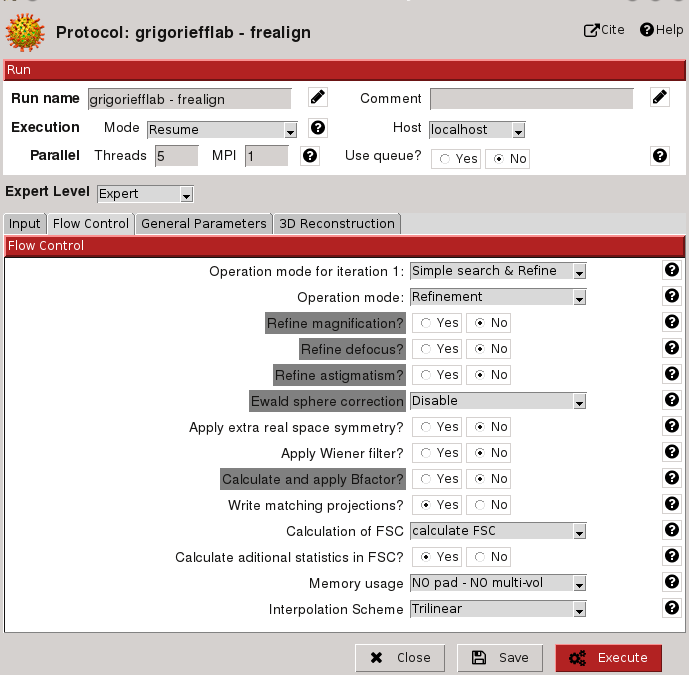
\includegraphics[width=0.75\textwidth]{{images/19.FrealignB}.png}
  \caption{Frealign parameters II}
  \label{fig:FrealignB}
 \end{figure}

  \begin{figure}
  \centering
  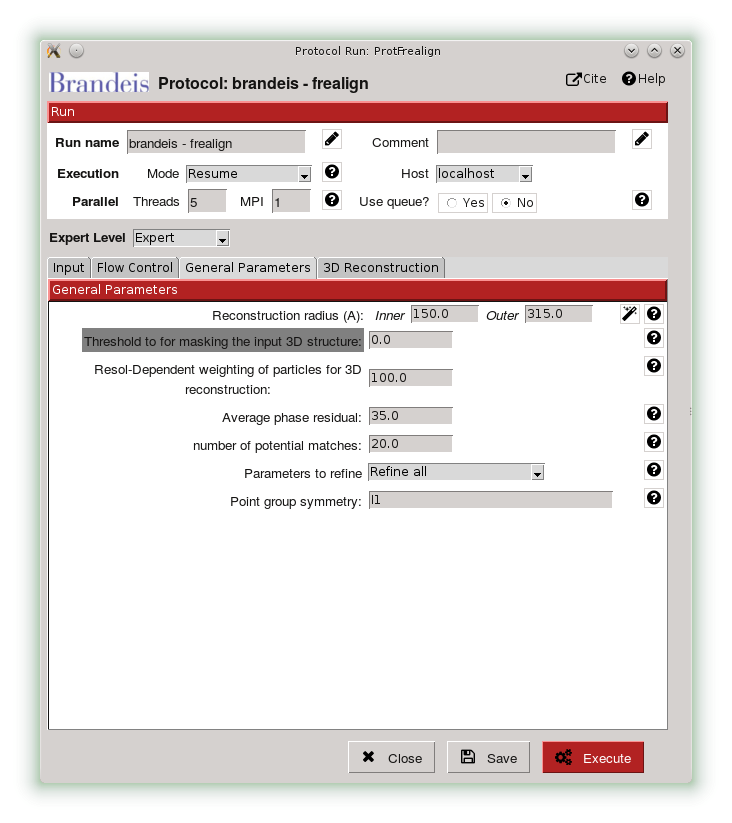
\includegraphics[width=0.75\textwidth]{{images/19.FrealignC}.png}
  \caption{Frealign parameters III}
  \label{fig:FrealignC}
 \end{figure}

  \begin{figure}
  \centering
  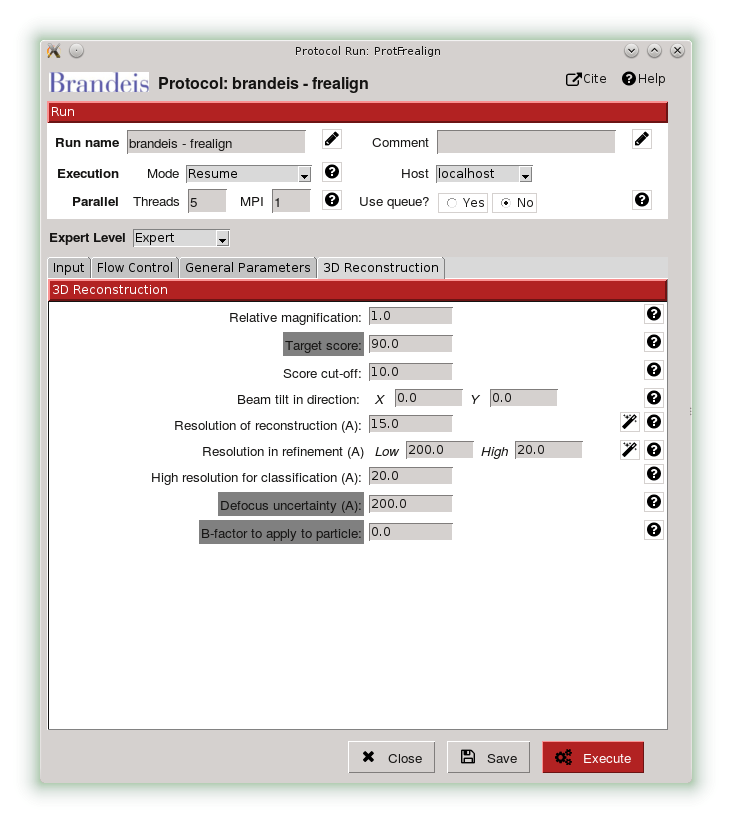
\includegraphics[width=0.75\textwidth]{{images/19.FrealignD}.png}
  \caption{Frealign parameters IV}
  \label{fig:FrealignD}
 \end{figure}

Again, in order to visualize the obtained results click on
\textbf{Analyze Results} button. You will see a GUI as the one shown in
figure (\ref{fig:FrealignViewer}).

 \begin{figure}
 \centering
 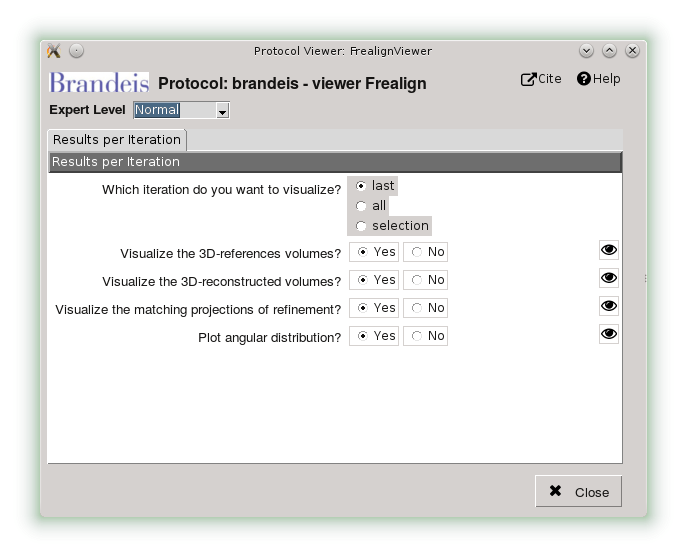
\includegraphics[width=0.75\textwidth]{{images/20.FrealignViewer}.png}
 \caption{Frealign viewer}
 \label{fig:FrealignViewer}
 \end{figure}

\bibliographystyle{apalike}
\bibliography{../tutorial_common/em.bib}

\end{document}
